

%%%
\subsection{Considérations préliminaires}

Soit un graphe $G=(S,A)$ tel que : $|S|=n$ et $|A|=m$ 
(avec $n,m\in\mathbb{N})$.

\noindent
Les sommets de $G$ sont numérotés de $0$ à $n-1$.

%%%
\subsection{Représentation par matrice d'adjacence}

\blue{
\begin{fDefinition}
La matrice d'adjacence du graphe $G$, soit $M$,  est une matrice 
booléenne de type $n\times n$ vérifiant : 
$$
M_{i, j} = \left\{
    \begin{array}{ll}
        1 & \mbox{si } i \mbox{ et } j \mbox{ sont adjacents} \\
        0 & \mbox{sinon}
    \end{array}
\right.
$$
\end{fDefinition}
}

Pour $i,j \in \{0, ..., n-1\}$, 
si $s_i$ est le $i$-ième sommet, 
et si $s_j$ est le $j$-ième sommet, 
alors : 
$$
M_{i, j} = 1 \iff (s_i, s_j)\in A
$$


%%%
\subsection{Représentation par liste d'adjacence}

\blue{
\begin{fDefinition}
La liste d'adjacence du graphe $G$, soit $\Succ$, est une liste indexée par les sommets de $G$, 
et telle que : 
$$\forall s\in S,~ \Succ(s)=\{s': (s,s')\in A\}$$
\end{fDefinition}
}
Autrement dit, $\forall s\in S$, 
$\Succ(s)$ est l'ensemble des sommets adjacents à $s$. 

%%%
\subsection{Exemple}

Soit le graphe $G=(S,A)$, défini par :
$$
\left\{
	\begin{array}{l}
		S=\{0, 1, 2, 3\}\\
		A=\{(0,2), (0,3), (1, 0), (2,1), (2,3), (3,1)\}
    \end{array}
\right.
$$

\noindent
Un tel graphe peut être représenté comme suit : 

\begin{center}
	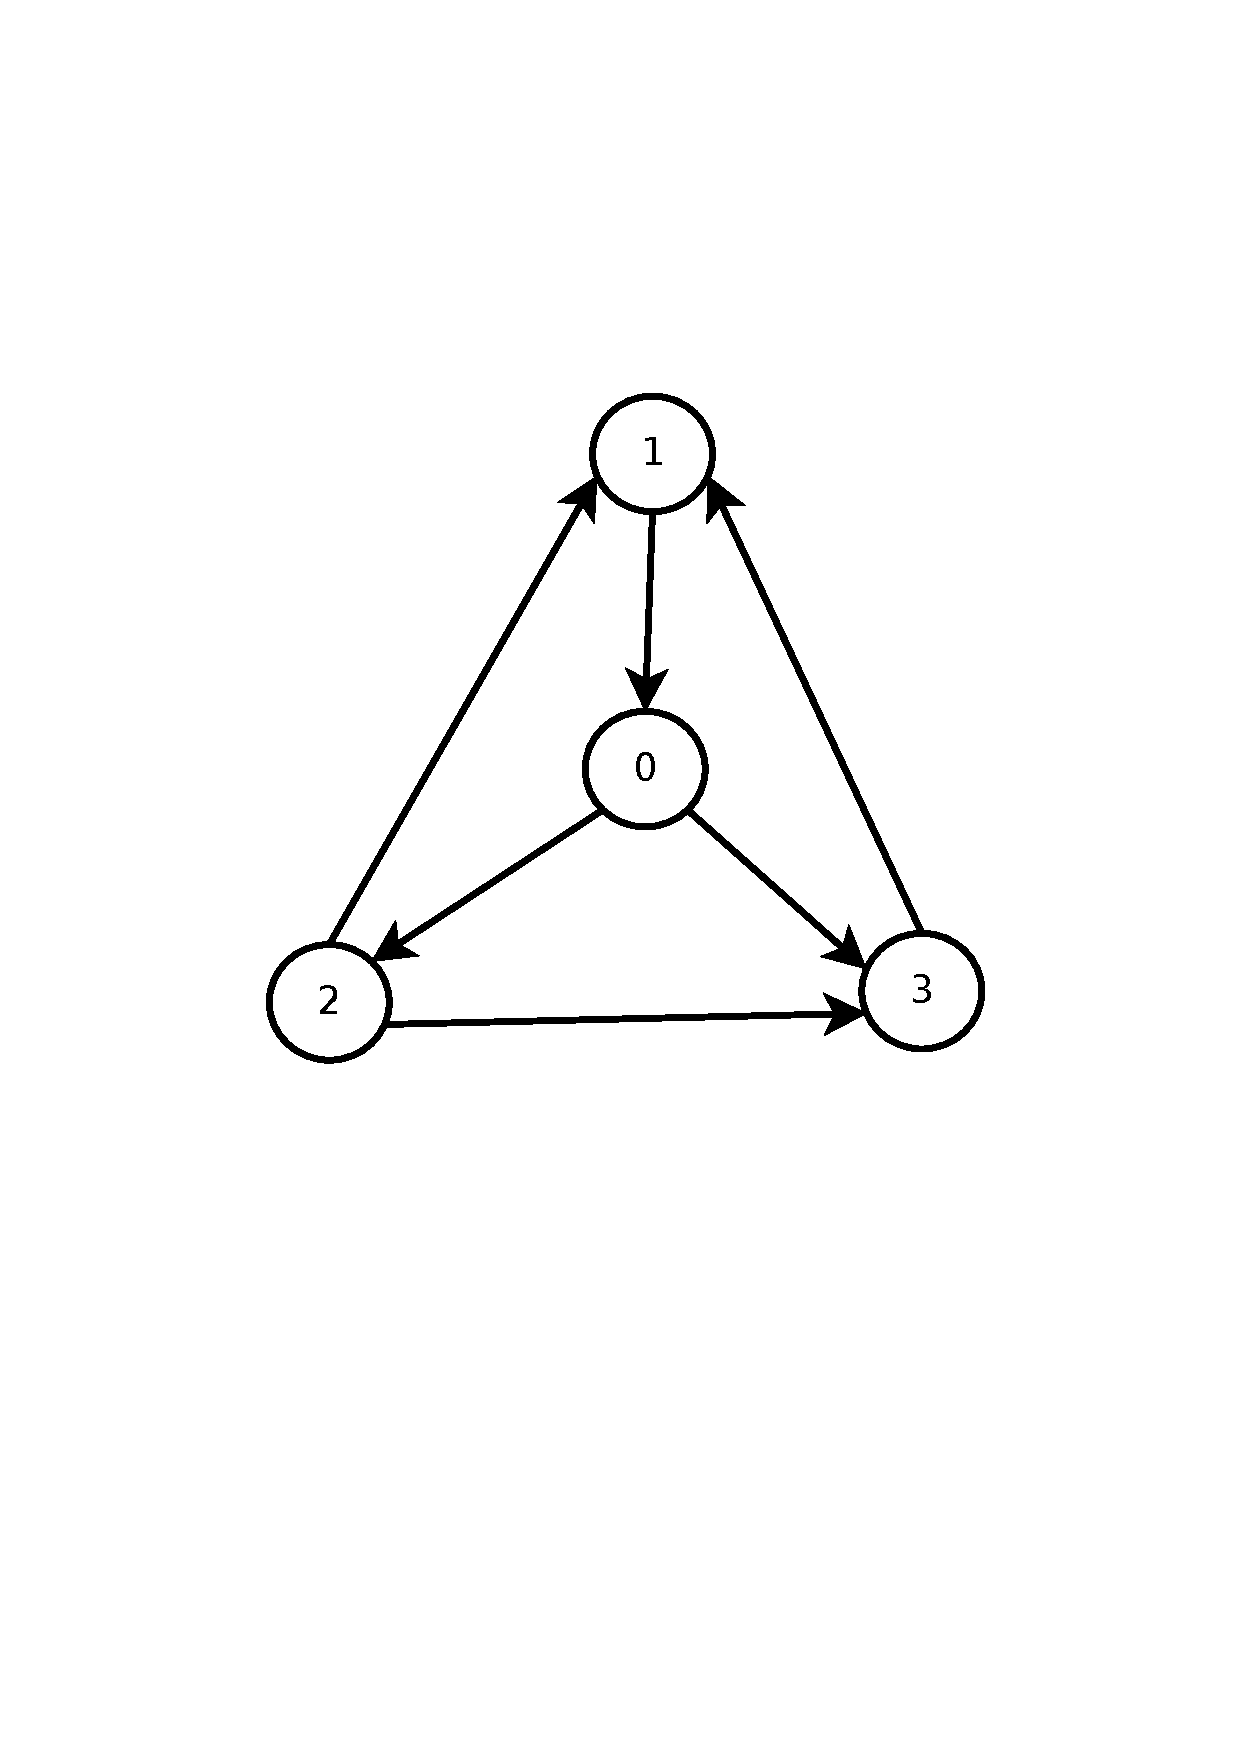
\includegraphics[scale=0.30]{exemple1_graphe.pdf}
\end{center}

Les représentatons par matrice et liste d'adjacence sont données ci-après.

\begin{center}
   \begin{tabular}{| c | c | }
     \hline
     \textbf{Matrice d'adjacence} 	& \textbf{Liste d'adjacence}\\
     \hline
$
\begin{pmatrix} 
 0 & 0 & 1 & 1 \\
 1 & 0 & 0 & 0 \\
 0 & 1 & 0 & 1 \\
 0 & 1 & 0 & 0 \\
 \end{pmatrix}
$
& 
	\begin{tabular}{|l|l|}
  	\hline
  	$0$ & $\{2, 3\}$ \\\hline
  	$1$ & $\{0\}$ \\\hline
  	$2$ & $\{1, 3\}$ \\\hline
  	$3$ & $\{1\}$ \\
  	\hline
   	\end{tabular}
   	
   \\
   \hline
   \end{tabular}
 \end{center}



%%%
\subsection{Espace mémoire}
\begin{center}
   \begin{tabular}{| l | l | }
     \hline
     \textbf{Matrice d'adjacence} 	& \textbf{Liste d'adjacence}\\
     \hline
     $O(n^2)$						& $O(n+m)$             	   \\ 
     \hline
   \end{tabular}
 \end{center}


%%%
\subsection{Complexité de quelques opérations}
\begin{center}
   \begin{tabular}{| l | l | l | }
     \hline
     \textbf{Opérations} 							& \textbf{Matrice d'adjacence} & \textbf{Liste d'adjacence} \\
     \hline
     Tester l'existence d'un arc $s\rightarrow s'$		& $O(1)$ 						& $O(|\Succ(s)|)$ \\
     \hline
     Retourner les sommets adjacents à un sommet		& $O(n)$ 						& $O(1)$ \\
     \hline
     Parcourir l'ensemble des arcs	 				& $O(n^2)$ 					& $O(m)$ \\
     \hline
   \end{tabular}
 \end{center}


\blue{
\begin{fLemma}
$$
\sum_{s\in S} |\Succ(s)| =  |A|
$$
\end{fLemma}
} 
 
%%%
\subsection{Choix d'utilisation}
\begin{itemize}
	\item D'une manière générale, on considère que si le graphe a  "peu" d'arêtes, il
	est plus intéressant d'utiliser une représentation par liste d'adjacence, plutôt que par
	matrice d'adjacence (qui contiendrait alors beaucoup de $0$).
	\item Mais si le graphe a "beaucoup" d'arêtes, il est plus intéressant d'utiliser 
	une matrice d'adjacence.
\end{itemize}

